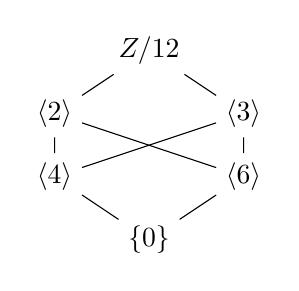
\begin{tikzpicture}[scale=0.8]
  \node (Z12) at (0,3) {\(\mathbb{Z}/12\)};
  \node (Z6) at (-1.5,2) {\(\langle 2 \rangle\)};
  \node (Z4) at (1.5,2) {\(\langle 3 \rangle\)};
  \node (Z3) at (-1.5,1) {\(\langle 4 \rangle\)};
  \node (Z2) at (1.5,1) {\(\langle 6 \rangle\)};
  \node (Z1) at (0,0) {\(\{0\}\)};
  \draw (Z12) -- (Z6) -- (Z3) -- (Z1);
  \draw (Z12) -- (Z4) -- (Z2) -- (Z1);
  \draw (Z6) -- (Z2);
  \draw (Z4) -- (Z3);
\end{tikzpicture}
